After the world wide web explosion at the ending of 1990's, Google has
emerged as one of the most significant web searching companies.
The novelty of Google was PageRank \cite{ilprints361}, an
algorithm counting the number of outgoing links of a webpage to determine its
importance. In order to apply the PageRank algorithm and form the
Google search results, first the webpage has to be scraped and
indexed. As of 2004 the raw size of the documents that had been
collected was more than 20 terabytes
\cite{Dean:2004:MSD:1251254.1251264}. Although the engineers at Google
have distributed and parallelized the algorithm, there were more tasks
that other teams have parallelized in a different way making it
difficult to maintain such a diverse codebase. That led them in 2004
to publish a paper about MapReduce, a generic framework to write distributed
applications that hide all the complexity of fault-tolerance, locality
awareness, load balancing etc.

MapReduce programming model borrows two very common functions from
functional programming, \emph{Map} and \emph{Reduce}. The \emph{Map}
function takes as input key/value pairs and produces as output a set
of key/value pairs as well. The \emph{Map} function is written by the
user and varies depending on the use case.

The \emph{Reduce} function, takes as input the
intermediate key/value pairs produced by \emph{Map} and merge them
together producing a smaller set of values. The \emph{Reduce} function
and the way it will merge the intermediate pairs is also provided by
the user.

A trivial example of the MapReduce programming model is that of
counting the occurrences of words in a text. The \emph{Map} function
takes as input a list of all the words in the text and emits a tuple
in the form \texttt{(word,1)}, where \texttt{word} is every word
parsed. The result of the \emph{Map} function is passed to the
\emph{Reduce} function which adds the value of the tuples with the
same key, in that case is the word. The result will be a list of
tuples where the key is all the words parsed from the text and the
value would be the occurrences of the word in the text.

Google provided a framework which took advantage of the locality
awareness of the already existing GFS and the MapReduce programming
paradigm. The execution overview of MapReduce is depicted in Figure
\ref{fig:mapreduce_execution_overview}.

\begin{figure}
\centering
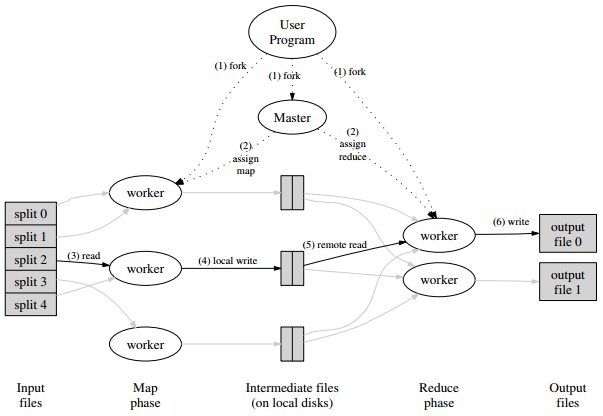
\includegraphics[scale=0.8]{resources/images/Background/mapreduce_exec_overview.png}
\label{fig:mapreduce_execution_overview}
\caption{MapReduce execution overview \cite{Dean:2004:MSD:1251254.1251264}}
\end{figure}

*easy to use, generic enough to fit in many problems, parallel, fault-tolerant